% This is "sig-alternate.tex" V2.0 May 2012
% This file should be compiled with V2.5 of "sig-alternate.cls" May 2012
%
% This example file demonstrates the use of the 'sig-alternate.cls'
% V2.5 LaTeX2e document class file. It is for those submitting
% articles to ACM Conference Proceedings WHO DO NOT WISH TO
% STRICTLY ADHERE TO THE SIGS (PUBS-BOARD-ENDORSED) STYLE.
% The 'sig-alternate.cls' file will produce a similar-looking,
% albeit, 'tighter' paper resulting in, invariably, fewer pages.
%
% ----------------------------------------------------------------------------------------------------------------
% This .tex file (and associated .cls V2.5) produces:
%       1) The Permission Statement
%       2) The Conference (location) Info information
%       3) The Copyright Line with ACM data
%       4) NO page numbers
%
% as against the acm_proc_article-sp.cls file which
% DOES NOT produce 1) thru' 3) above.
%
% Using 'sig-alternate.cls' you have control, however, from within
% the source .tex file, over both the CopyrightYear
% (defaulted to 200X) and the ACM Copyright Data
% (defaulted to X-XXXXX-XX-X/XX/XX).
% e.g.
% \CopyrightYear{2007} will cause 2007 to appear in the copyright line.
% \crdata{0-12345-67-8/90/12} will cause 0-12345-67-8/90/12 to appear in the copyright line.
%
% ---------------------------------------------------------------------------------------------------------------
% This .tex source is an example which *does* use
% the .bib file (from which the .bbl file % is produced).
% REMEMBER HOWEVER: After having produced the .bbl file,
% and prior to final submission, you *NEED* to 'insert'
% your .bbl file into your source .tex file so as to provide
% ONE 'self-contained' source file.
%
% ================= IF YOU HAVE QUESTIONS =======================
% Questions regarding the SIGS styles, SIGS policies and
% procedures, Conferences etc. should be sent to
% Adrienne Griscti (griscti@acm.org)
%
% Technical questions _only_ to
% Gerald Murray (murray@hq.acm.org)
% ===============================================================
%
% For tracking purposes - this is V2.0 - May 2012

\documentclass{sig-alternate}

\usepackage{url,subfigure}
\usepackage[subtle]{savetrees}

\permission{Copyright is held by the International World Wide Web Conference Committee (IW3C2). IW3C2 reserves the right to provide a hyperlink to the author's site if the Material is used in electronic media.}
\conferenceinfo{WWW 2015 Companion,}{May 18--22, 2015, Florence, Italy.} 
\copyrightetc{ACM \the\acmcopyr}
\crdata{978-1-4503-3473-0/15/05. \\
http://dx.doi.org/10.1145/2740908.2743975}

\begin{document}
%
% --- Author Metadata here ---
\conferenceinfo{SOCM2015}{2015, Florence, Italy}
%\CopyrightYear{2007} % Allows default copyright year (20XX) to be over-ridden - IF NEED BE.
%\crdata{0-12345-67-8/90/01}  % Allows default copyright data (0-89791-88-6/97/05) to be over-ridden - IF NEED BE.
% --- End of Author Metadata ---

\title{Social Personal Data Stores: \\ the Nuclei of Decentralised Social Machines}

%
% You need the command \numberofauthors to handle the 'placement
% and alignment' of the authors beneath the title.
%
% For aesthetic reasons, we recommend 'three authors at a time'
% i.e. three 'name/affiliation blocks' be placed beneath the title.
%
% NOTE: You are NOT restricted in how many 'rows' of
% "name/affiliations" may appear. We just ask that you restrict
% the number of 'columns' to three.
%
% Because of the available 'opening page real-estate'
% we ask you to refrain from putting more than six authors
% (two rows with three columns) beneath the article title.
% More than six makes the first-page appear very cluttered indeed.
%
% Use the \alignauthor commands to handle the names
% and affiliations for an 'aesthetic maximum' of six authors.
% Add names, affiliations, addresses for
% the seventh etc. author(s) as the argument for the
% \additionalauthors command.
% These 'additional authors' will be output/set for you
% without further effort on your part as the last section in
% the body of your article BEFORE References or any Appendices.

% of EIGHT authors. SIX appear on the 'first-page' (for formatting
% reasons) and the remaining two appear in the \additionalauthors section.
%
% You can go ahead and credit any number of authors here,
% e.g. one 'row of three' or two rows (consisting of one row of three
% and a second row of one, two or three).
%
% The command \alignauthor (no curly braces needed) should
% precede each author name, affiliation/snail-mail address and
% e-mail address. Additionally, tag each line of
% affiliation/address with \affaddr, and tag the
% e-mail address with \email.
\numberofauthors{6} %  in this sample file, there are a *total*
% of EIGHT authors. SIX appear on the 'first-page' (for formatting
% reasons) and the remaining two appear in the \additionalauthors section.
%
% You can go ahead and credit any number of authors here,
% e.g. one 'row of three' or two rows (consisting of one row of three
% and a second row of one, two or three).

% The command \alignauthor (no curly braces needed) should
% precede each author name, affiliation/snail-mail address and
% e-mail address. Additionally, tag each line of
% affiliation/address with \affaddr, and tag the
% e-mail address with \email.
% 1st. author
% all the authors: eMax, DMR, Amy, DS, Nigel
\author{
\alignauthor Max Van Kleek\\
        \affaddr{Web and Internet Science}\\
        \affaddr{University of Southampton, UK}\\
        \email{emax@ecs.soton.ac.uk}
\alignauthor Daniel A. Smith\\
        \affaddr{Web and Internet Science}\\
        \affaddr{University of Southampton, UK}\\
        \email{ds@ecs.soton.ac.uk}
% 2nd. author
\alignauthor Dave Murray-Rust\\
        \affaddr{School of Informatics}\\
        \affaddr{University of Edinburgh, UK}\\
        \email{d.murray-rust@ed.ac.uk} 
\and 
\alignauthor Amy Guy\\
        \affaddr{School of Informatics}\\
        \affaddr{University of Edinburgh, UK}\\
        \email{Amy.Guy@ed.ac.uk}
\alignauthor Kieron O'Hara\\
        \affaddr{Web and Internet Science}\\
        \affaddr{University of Southampton, UK}\\
        \email{kmo@ecs.soton.ac.uk}
\alignauthor Laura Dragan\\
        \affaddr{Web and Internet Science}\\
        \affaddr{University of Southampton, UK}\\
        \email{lcd@ecs.soton.ac.uk}
\and
\alignauthor Nigel R. Shadbolt\\
        \affaddr{Web and Internet Science}\\
        \affaddr{University of Southampton, UK}\\
        \email{nrs@ecs.soton.ac.uk}
}
% There's nothing stopping you putting the seventh, eighth, etc.
% author on the opening page (as the 'third row') but we ask,
% for aesthetic reasons that you place these 'additional authors'
% in the \additional authors block, viz.
\date{1 February 2015}
% Just remember to make sure that the TOTAL number of authors
% is the number that will appear on the first page PLUS the
% number that will appear in the \additionalauthors section.

\maketitle


\begin{abstract}
Personal Data Stores are among the many efforts that are currently underway to try to re-decentralise the Web, and to bring more control and data management and storage capability under the control of the user.  Few of these architectures, however, have considered the needs of supporting decentralised social software from  the user's perspective. In this short paper, we present the results of our design exercise, focusing on two key design needs for building decentralised social machines: that of supporting heterogeneous social apps and multiple, separable user identities. We then present the technical design of a prototype social machine platform, INDX, which realises both of these requirements, and a prototype heterogeneous microblogging application which demonstrates its capabilities.
\end{abstract}

% A category with the (minimum) three required fields
\category{H.4}{Information Systems Applications}{Miscellaneous}
%A category including the fourth, optional field follows...
%\category{D.2.8}{Software Engineering}{Metrics}[complexity measures, performance measures]

% \terms{Personal }

\keywords{Decentralising the Web, Social Machines, Software Architectures, Privacy}

\section{Introduction}

The increasing centralisation of the Web remains the greatest threat to its continued existence as a democratic and ubiquitous shared medium of communication~\cite{redecent}. Although originally designed as a decentralised system to ensure longevity and sustained fair and equal access to all that use it, today the Web has become a highly centralised environment, dominated by very large institutions (such as Facebook, Google, Weibu, Baidu, and Twitter, among others) that each control all of the traffic that flows within their respective borders.  The result is that such institutions harbour a disproportionately large percentage of Web traffic, and, in turn, exercise an unprecedented degree of control over its governance and operation.  Moreover, this control extends not just to the operation of the sites themselves, but also over the personal data that people are voluntarily pouring into them, whether they pertain to one's online social network activities, or, increasingly, the contents of one's personal information collections shifting from desktops into ``the cloud''.

The centralisation has made service providers the \emph{de facto} locus of control for both user data and interaction.  Whenever a service provider wishes to change some functionality of its service, such as to roll out a new feature, it is within their power to simply roll out changes, and the users of the platform essentially are usually quite powerless to do anything about it regardless of their preferences or needs.  This is not good for users for multiple reasons; first, it disenfranchises people from the choice to have the features they want, or in the ways that they have grown accustomed to. Secondly, the sudden and unexpected roll out of new designs and features often results in people perceiving changes in more negative a light, ultimately slowing and stagnating innovation.

%  When such a change effectively makes it impossible for a person to conduct the day-to-day activities she or he once relied on, this itself can be disruptive to a person's life.  

This relates to social machines because the Web itself has proven the most profoundly transformative social machine in the history of humanity, fundamentally enabling currently over 60\% of the world's population to work, collaborate, meet more effectively, interact socially and enjoy new forms of recreation.  Within the Web, studies of differences among individual ``sub'' social machines, such as social networking platforms, online communities and the like, have shown that subtle differences among  each have greatly shaped the resulting community around them and the ways people use and interact through them~\cite{ross2010person}.  The implications of these observations is that even relatively minor details of next-generation Web based social machines will likely have a tremendous impact on the ways people will interact with and through them.  As a result, we feel that it is very critical that requirements and technical design decisions be driven by an understanding of what makes today's Web based social machines effective, sustain, as well as of where they fall short or how they fail.

In this paper, we extend a line of work we have introduced previously (\cite{van20147,van2014future,van2012decentralized})  pertaining to investigating the fundamental idea of giving end-users of the Web more sophisticated data management capabilities ``at the edge'', ie.. on the physical computing device(s) that they own and/or control.  In particular, we focus on one very specific aspect of personal data store work pertaining to social machines: the problem of building social platforms in fully decentralised Web environments.   

% Although this may seen contradictory to the pervasive trend towards moving physical computing capability into virtualised ``cloud'' environments, we refer less about the physical versus virtual nature of the compute infrastructure than \emph{whom} it is controlled by, and moreover, the extent to which end-users can define the operations therein. Although the idea of the \emph{personal data store} has been proposed many times in the past, we argue that research in PDSes has been fundamentally limited thus far in at least three ways; first, the assumption that the PDSes are singular, monolithic repositories for ``all'' one's personal data; second, that PDSes are in some sense, personal not \emph{social}; and third, have not yet considered aspects of long-term maintenance and use, in particular pertaining to \emph{data evolution} and integration.

\section{Background}

Before the rise of massive social networks and platforms, decentralised operation was the norm; from before the Web, operating systems like UNIX supported a number of utilities for connecting with other hosts in ways that could be either seen as primitive social software (e.g. UNIX Talk), or used to build social software (e.g. telnet for MUDs and MOOs). Even after the growth of massive providers, being able to connect multiple disparate platforms was seen as a reason to build protocols like Jabber/XMPP\cite{saint2005streaming} or to use a common social protocol such as IRC.  However, the use of such protocols seems to be declining, with the major platform providers Google and Facebook both terminating support for XMPP on their Talk and Facebook chat services, for example, thereby, for the moment, eliminating the possibility of bridging communications across them.

Meanwhile, as if by Newton's third law, this trend towards centralisation has compelled open source hackers and enthusiasts, driven by increased concerns over privacy and dislike of increased control, towards build re-building social software that is decentralised.  Such efforts themselves have now become so distributed and widespread that a number of different indices have sprung up to track these efforts (e.g. on Wikipedia\footnote{Comparison of software for distributed social networking \url{en.wikipedia.org/wiki/Comparison_of_software_and_protocols_for_distributed_social_networking}}, and GitHub Alternative-Internet\footnote{Alternative Internet: \url{github.com/redecentralize/alternative-internet}}), and the IndieWeb movement\footnote{IndieWeb \url{indiewebcamp.com/}}. 

These systems can be roughly divided into three classes corresponding to their degree of decentralised operation.  The first category, containing possibly the largest number of independent web projects, are those that are simply standalone servers intended for operation and use by the end-user.  In this basic category, services are in essence entirely centralised, but are made to be run by the end-user (on his or her own computational substrate) instead of by a third-party, thus providing for entirely private operation, maintenance and control.  The second category extends the first with interoperability through the use of common, standardised data representations and APIs to enable interchange among heterogeneous systems.  Such social protocols include \textbf{Activity Streams}\footnote{Activity Streams specification \url{http://activitystrea.ms/}}, which are a syndicate format for feeds from social networking services, as well as \textbf{XMPP}, \textbf{OpenID}, \textbf{OAuth}, and \textbf{WebID}, among other standard formats for identity and data exchange.  A third category, in contrast to the first two, implements social applications in a distributed, rather than federated, fashion over an open set of participating nodes, typically end-users themselves or volunteers.  This is the philosophy of applications such as \textbf{Bittorrent}, \textbf{Freenet}, \textbf{IPP}, \textbf{Tor}, \textbf{Twister}\footnote{Twister, A Fully Decentralised Microblogging Client - \url{http://twister.net.co/}}, and \textbf{Bitcoin}; in some, such as Bittorrent, Freenet and Twister, participation requires contribution of the computational, network and storage resources required to keep the service running; while in others, such as Tor and Bitcoin, one can use a service without contributing, i.e. serving as a Tor relay/exit node, or Bitcoin Miner.

A second dimension on which these systems differ is the extent to which they are bespoke to a particular application.  Many have 'baked in' functionality specific to emulating the biggest social applications today, roughly comprising interfaces for social networking (e.g. activity status update and photo/item sharing), microblogging, blogging, forums, and file/data item storage and hosting.  Others, such as Tor, are purely generic, providing specific capabilities for building social applications, such as  anonymous data routing and connectivity.  Still other examples exist that are the creation of new social applications by co-opting others; an example of this  is the a proof-of-existence service\footnote{Proof of Existence - \url{www.proofofexistence.com}} that uses the Bitcoin blockchain to prove that particular information was known by a party at a particular relative time.

Finally, perhaps the the most well known distributed social networking project is Diaspora\footnote{Diaspora - \url{joindiaspora.com}}, once hailed as the 'decentralised Facebook-killer'~\cite{verge}.  Its architecture is most relevant for the discussion in this paper, because it, like ours, is more decentralised than distributed; anyone with appropriate network and computational resources can host their own ``pod'' server, and engage in Facebook-like social networking activities with others either within the same pod or those hosted on others.  Unlike Diaspora, however, which has a bespoke social networking application baked into it, our architecture is designed to be a generic substrate for building decentralised social applications, as we describe next.

\section{Designing a Platform for Decentralised Social Machines}

Given the varied and abundant efforts at decentralising the Web just described, we wished to know whether the capabilities envisioned by such efforts would align well with the potential design requirements for future social machines~\cite{hendler2010semantic}.  To identify such requirements, we undertook a brainstorming activity with two experts on personal data architectures and one on Web-based social machines.  Out of the twelve design requirements we derived, six remained unfulfilled by any of the proposed decentralised projects; out of these, we focus on two which are the most relevant to social aspects of future social machines.

\subsection{Heterogeneous Social Software}

One of the key goals of the efforts at decentralising the web is to put people ``in control'' of their social software. But the implications of such a simple statement could be many; one, for example, might be to ``control'' data generated in social interactions (e.g., one's Tweets, status updates, Instagrams), which we interpret to be able to access, use, appropriate, such content as one wishes, indefinitely.  At this level, several of the existing personal data stores already fulfil this need well; many PDSes interface with existing social platforms on the Web through APIs, to make and store copies of the individual's own content with the objective of storing this content for safekeeping.

Another interpretation is that end-users should control the look, feel and functionality of their social software.  One way that this has been achieved in the past is the use of third-party apps that provide different interfaces and, in some cases, add functionality, to the big Web social platforms. However, nearly all of the major social platforms today seem to be shifting towards restricting and denying third-parties from doing so, for the purpose of exercising more control, often under the auspices of protecting users from malicious software~\cite{shutdown}. As a result, in the foreseeable future, it seems that the major social platform providers will continue to mandate use of their genuine apps and clients only, eliminating user choice in interface or features.

In a decentralised setting, however, such mandating use of a single client is not only unlikely, but also potentially harmful to widespread adoption.  Therefore, we believe that we will see a rise of \emph{heterogeneous social software}, consisting of what might be thought of as an ecosystem of ``apps'' today that support social interaction despite their not being the same. 

The standard method for allowing heterogeneous clients to interact is establishing a common protocol for interaction, such as XMPP, Activity Streams, as mentioned earlier. Indeed, the many aforementioned systems already do this. However, this is a conservative approach that slows innovation, because the vocabulary has to be established essentially \emph{a priori} to creating applications, and, applications must fully comply with the protocol(s) in order for systems to be able to interact.  Thus, in such scenarios protocol designers have incredible power by essentially dictating how a social machine is to work, yet, based on previous examples, are rarely involved in the process of designing apps themselves.

An alternative approach is to provide support for more organic interoperability by allowing app designers to extend or forge new data representations themselves, and then, to promote interoperability, support others' use of their representations though representational alignment. We propose that such support could easily be provided by the social machine platform framework, and describe this functionality in the next section.  

With this approach, barriers between the activities supported by individual social machines can be arbitrarily blurred by social app designers; if an app maker adds a new kind of social action to an existing data type, for example, to support 'retweeting' instagrams, they are free to do so; and any new apps can choose to support this action or ignore it.

\subsection{Identities, Pseudonyms and Personas}

% Quick notes, Amy will attempt to write up first thing in the morning if someone else doesn't get there first..
%people have complex identity behaviours; many different reasons.
%need capacity for multiple versions of self online.
%people circumvent technical or policy restrictions or repurpose features of a system to achieve this.
%use different systems for different things, or multiple accounts on same system.
%share personas across platforms and communities aka across social machines.
%need understanding of the context in which a version of themselves is visible - what parts are visible to whom and when.
%how to control this and retain user confidence, across different systems?
%how to select a persona to authenticate with?
%how to ensure users can express their online identity as they like?
%when a social machine spans multiple technical systems, how to interoperate identity and community norms?


We have used the term \emph{personal} data store extensively, but without fully exploring what personal really means. As they live their lives, individuals tend to carry out a variety of different tasks and activities, for different reasons, with different groups of people. This is as true online as it is offline, but with some differences. In a recent study, we discovered that a majority of people who use the Web perform some kind of identity separation online, in an effort to control the information they choose to make available about themselves in particular contexts~\cite{turnip}.  Our study also found that people become frustrated when they unwittingly lose control of their personal data as it is propagated throughout systems by algorithms and architectures of which they are not aware or do not fully understand. Examples of this include changes to Facebook privacy settings which suddenly expose sensitive status updates to work colleagues, or forced linking of Google+ and YouTube accounts which reveals real names and locations of users to aggressive commenter.

Unintentional spreading of personal information from one group, community or network to another can result in collapsing of social contexts~\cite{marwick2011tweet}, which potentially has serious implications for the individual involved.  People take steps to mitigate against this in many different ways, as described in~\cite{turnip}, including lying about personal data when they feel it is not required; keeping distinct social media accounts to separate work and personal affairs, or to post different types of content to; clustering sets of accounts together under a single pseudonym to maintain consistency without exposing their offline identity; exaggerating or omitting aspects of themselves to perform for or better integrate with a particular community; keeping `safe' social media accounts for their friends and family whilst expressing their true feelings from alternative `secret' accounts. 

Yet, service providers continue to develop more sophisticated methods to counteract this behaviour, in an effort to more accurately track individuals for advertising purposes, and to enforce real-name policy routines.  Click-stream profiling and Deep Packet Inspection (DPI) have become increasingly commonplace~\cite{bendrath2011end,collins2009privacy}, which make it extremely difficult for end-users to avoid being re-identified. 

Existing work on Personal Data Stores largely fails to account for the need for multiple identities, effective separation of roles and anonymity, and to prevent unwanted tracking and click-stream profiling.  Some of the most prominent PDSes, such as Mydex, for example, aim to serve as 'trusted Identity Brokers which certify that people are who they ``truly claim to be'' (fulfilling a Versign-like role)~\cite{heath2013digital}, which is completely contrary to current Web users'  most frequent needs when protecting themselves online.  Even systems like Diaspora and Buddycloud, which support standard distributed ID protocols such as OpenID, fundamentally assume that the individual has and maintains a single profile and identity which they disclose to all services equally; a practice that does not reflect the reality of what people do, nor the various reasons for doing so.

In order to support people's needs surrounding their privacy, we sought to design a system to actively support the kinds of practices people already perform when interacting with the many large platforms on the Web.  As we describe later, INDX aims to actively support the creation and effective management of as many separate identities as the person desires, and to permit fluid switching of identities as they switch from provider to provider.  More critically, we sought to help protect users from unwanted context collapse through the use of counter-surveillance techniques that are even able to defeat most forms of clickstream and DPI.  These methods remain an area of active research for us, and are described in greater detail in a separate paper~\cite{murray2014social}.

% I'll try to get to this, but might not make it (DMR)

\section{INDX: A Decentralised Social Machine Platform}

In this section, we describe our progress with a prototype Social Personal Data Store (SPDS) platform
in which we first sought to realise the functionality pertaining to the aspects just described, as they
were most germane to building social machines.  To do this, we extended the INDX Personal Data Store~\cite{van2012decentralized}
which was a fairly traditional centralised PDS that end-users of the Web could run on their personal compute
hardware and use to securely store and archive content from all over the Web.  

From this as a starting point, we added two capabilities: heterogeneous schema management, for the purposes
of allowing multiple social apps to easily exchange information with one another despite having different
data schemas and representations, and, second, multiple identity management capabilities in support of
the aforementioned perceived need to help users manage multiple identities and personas online. 
We next describe the technical details of each.

\subsection{Heterogeneous Social App Data Mapping}

\begin{figure}[t!]
 	  \begin{center}
        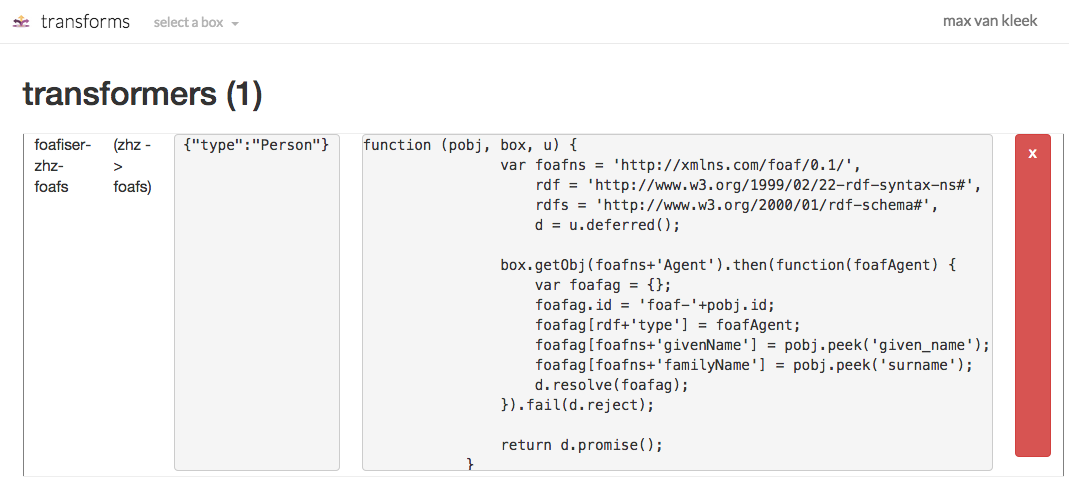
\includegraphics[width=0.50\textwidth]{transformer}
       \end{center}
    \caption{%
        Transformer engine loaded with CIMBA-TIMON microblogging bidirectional transform rule from INDX representation to CIMBA.
    }%
  \label{fig:transform}
\end{figure}


As mentioned earlier, unlike in centralised Web settings where social platforms can fully establish and dictate the ways end-user clients interact with them, in an open, decentralised setting, there will be, in general, no such ability to fully control the constituents in the network.  Therefore, supporting effective exchange among the heterogeneous constituents is a priority.  Fortunately, the Web has standardised, at the protocol level (e.g. HTTP, WebSockets, etc) how information should be exchanged; however, it does not dictate the forms and representations of the data exchanged. 

Thus, for INDX, we focused on the problem of achieving effective heterogeneous structured data exchange.  To do this, we adopted the pragmatic approach: a rule engine that is capable of transforming any simple structured data representation to another, through the use of modular rulesets.  Modularity ensured that, as new social apps were introduced, or old ones were modified or improved, the data representations could be easily and appropriately made compatible simply by updating the corresponding ruleset. 

Rule-based data transformation is a technique that has been applied to systems for decades; our contribution is simply, first, to determine whether this technique would afford sufficient flexibility to permit heterogeneous applications to be made to speak to each other, and second, whether the complexity of managing modular rulesets could be made sufficiently manageable for end-users.   With respect to technical implementation, we considered a number of existing rule languages and engines, including RDFS and OWL reasoners; for the first prototype, we opted for a simpler (less expressive) rule language based on INDX's query language, so that queries could be both succinctly expressed in terms of a INDX's native data format, and so that the satisfaction of rules could be performed directly within INDX's core Postgres engine itself.

\begin{figure}[t!]
 	  \begin{center}
        \subfigure[CIMBA]{%
            \label{fig:fb}
            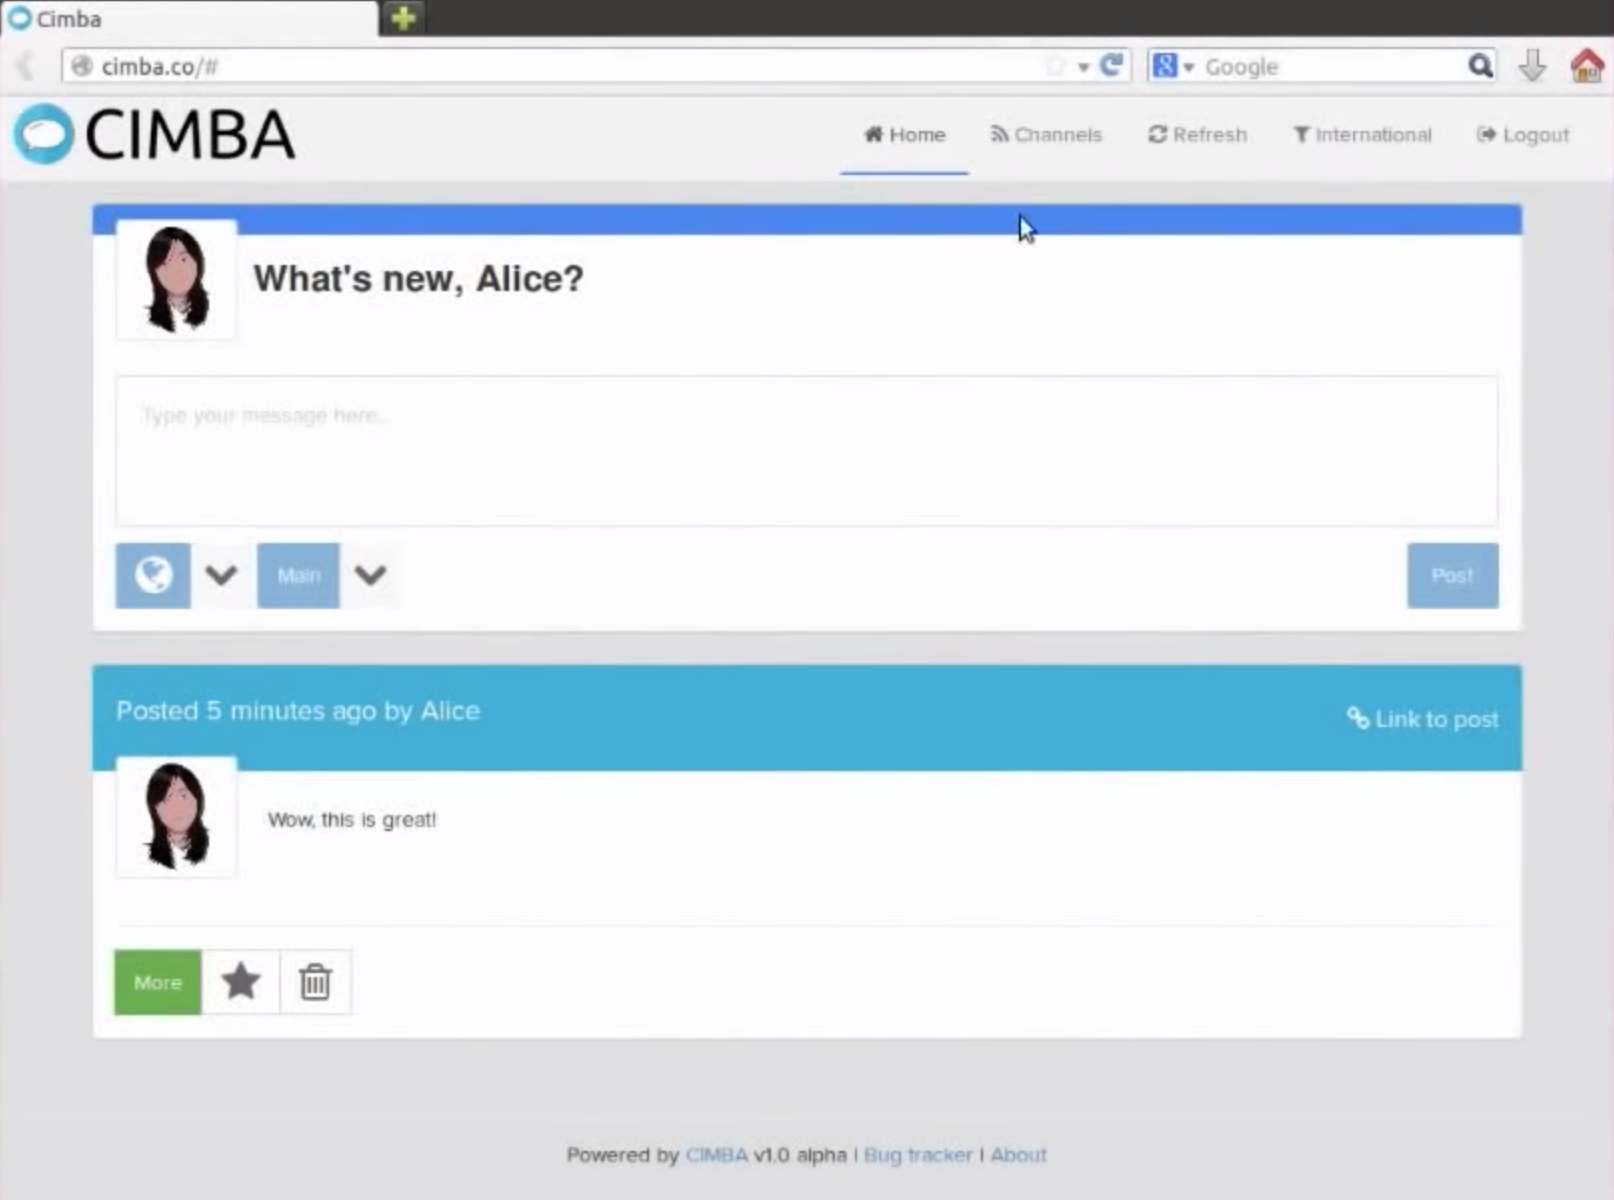
\includegraphics[width=0.48\textwidth]{cimba}
        }\\
        \subfigure[TIMON]{%
          \label{fig:twitter}
          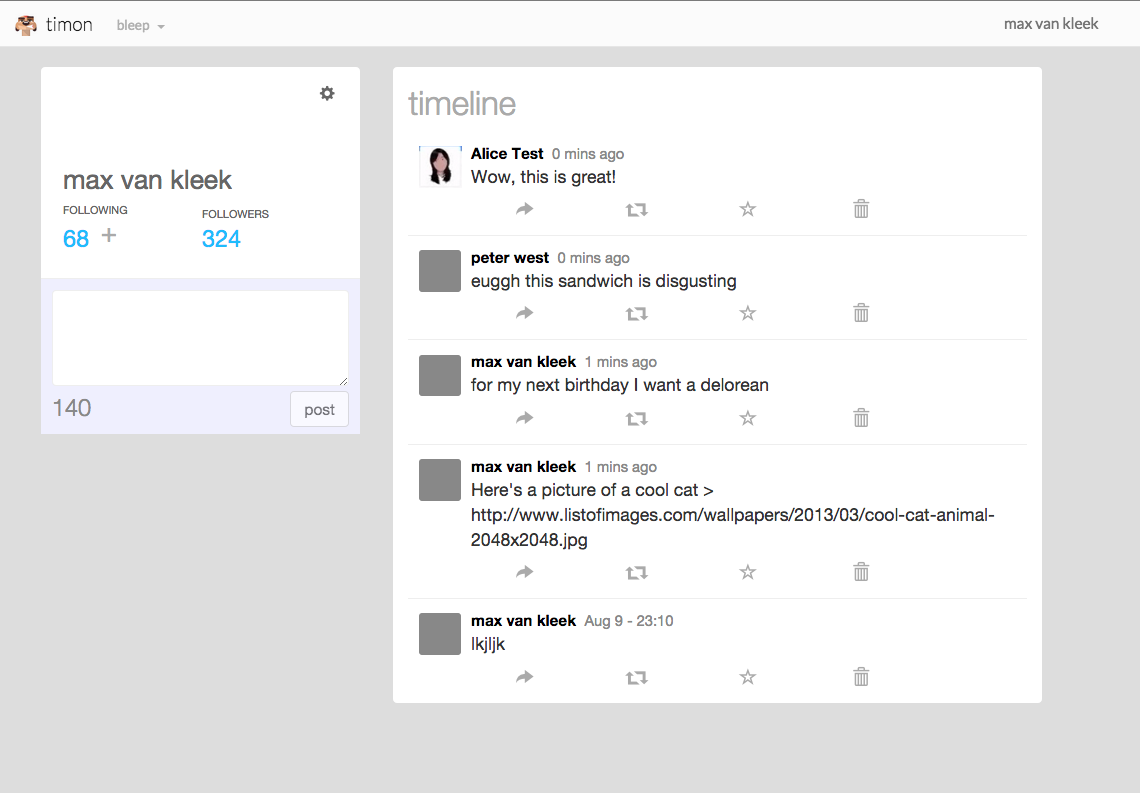
\includegraphics[width=0.48\textwidth]{timon}
        }        
    \end{center}
    \caption{%
        Original CIMBA client, top, running on the Linked Data Platform, communicating transparently with INDX's TIMON (bottom) via the schema-translation rule engine.
    }%
  \label{fig:timon}
\end{figure}


Figure \ref{fig:transform} displays a patching rule for INDX's \emph{TIMON} adaptive microblogging application to communicate with the CIMBA linked-data microblogging platform~\cite{sambracimba, presbrey2014linked}. In the figure, the left-hand query represents a native INDX query which specifies the domain of the transform; the right-hand side represents the equivalent transformed representation that CIMBA expects. Note that CIMBA uses RDF, while INDX uses a JSON-like object format; yet, because JSON can express a superset of RDF, the rule language can effectively generate RDF. Note that, in its simple initial implementation, rules are uni-directional; therefore two symmetric rules are required for bi-directional integration. We are intending to make the rule-engine able to run rules in reverse (by using the output transformation syntax as a query for reverse transforms) in the next iteration of the prototype.  The current versions of CIMBA and TIMON inter-operating are visible in Figure \ref{fig:timon}.

The advantage of this approach over simply adopting a common vocabulary (such as done by Buddycloud or Diaspora) is flexibility; while a particular format or ontology might be standard today, a new application may include new information that poorly suits the schema, thus outgrowing it.  As can be seen in the example, CIMBA itself uses two standard vocabularies intertwined, FOAF~\cite{brickley2012foaf} and SIOC~\cite{champin2010sioc}.  Not only can our approach directly support the particular peculiar use of these two standard vocabularies, but it can also easily be bridged, via a separate ruleset, to communicate with Diaspora as well, which uses Activitystreams, OStatus and other vocabularies.  

\subsection{Multiple Identities and Counter-surveillance}

%Enforcing separation of roles and identities can be tricky even in the offline world, but remains a routine practice nonetheless; thus we brainstormed fundamental ways that the platform could support end-users to make the process both more naturally mirror the offline world and to reduce the effort required in doing so.  

Fundamentally, we aim to have INDX support end-users' desires in keeping identities as separate as they wish, with the properties they please.  The first feature we implemented was to support the creation and maintenance of multiple, separate identities and social networks; INDX facilitates creation of as many  identities as the user wants.  Each of these identities can be adapted to popular distributed ID representations (at this point, comprising only OpenID or WebID, although more are planned) to facilitate their use with third parties.  In addition to supporting distributed ID protocols, each identity can be associated with sessions/session cookies and principals created on closed Web-based platform identities.   What explicit association between identities and principals does, thus, is allow the platform to help manage switching among identities at appropriate times, to aid in preventing accidental context overlap.  For example, by storing credentials separately and by third party service, INDX can allow an individual to choose which identity to present whenever interacting with a third-party service. Eventually, we wish to add predictive algorithms to make this selection easier or even automatic.

The second built-in set of functionality we see as integral to supporting effective identity separation in INDX pertains to helping users to avoid being tracked without their consent, particularly using DPI, user agent profile and click-stream profiling.  Such methods could cause service providers to infer a person's other identities, for example, defeating their ability to keep identities separate.  Towards this end, thus, INDX makes default all connections to third parties to use Tor~\cite{tor} to ensure that connection and packet-based profiling remains impossible.  As a second measure, INDX integrates via a browser-plugin to provide coordinated user-agent randomisation for third parties corresponding to particular identities; for example, when interacting with Facebook under Identity 1, INDX might set the browser user agent to present itself as Safari running on OS X, while, with Identity 2 IE11 on Windows 8.1.  While such counter-surveillance measures are still rudimentary compared to the level of sophistication being applied by service providers to track their users, they represent a first step in a programme to shift user control back to the user.

% In order to support the need to maintain multiple identities, personas and disjoint social networks, as well 
% 


\subsection{Practical Considerations w/ Connectivity}

\begin{figure}[t!]
 	  \begin{center}
        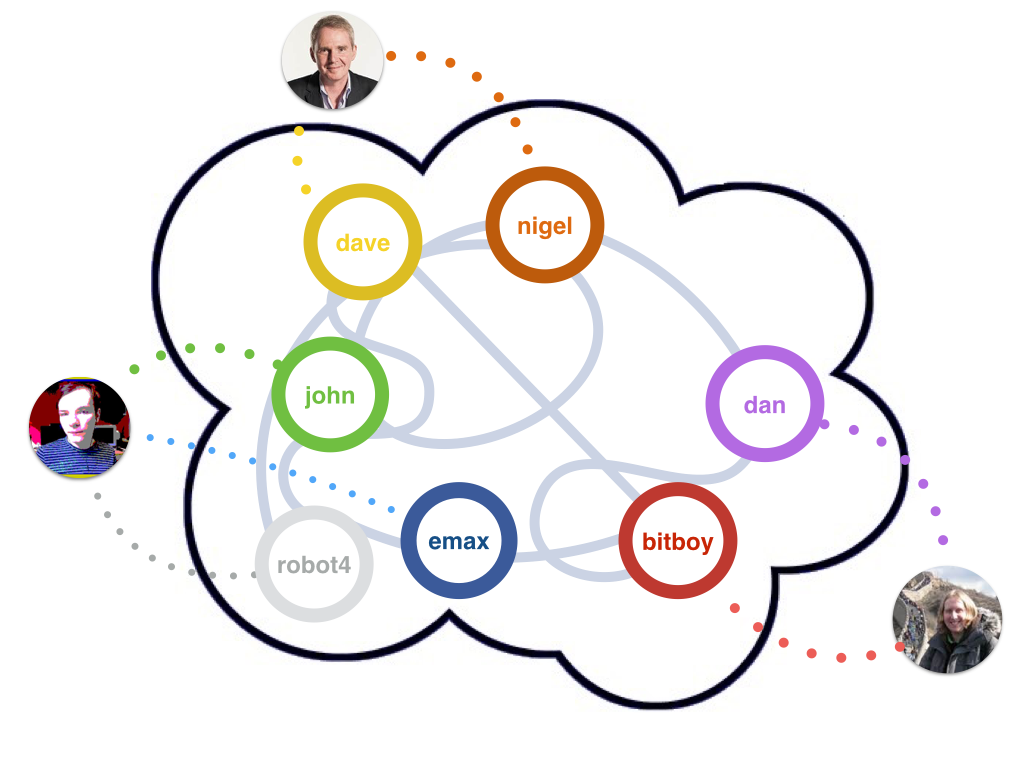
\includegraphics[width=0.50\textwidth]{tor}
       \end{center}
    \caption{%
        Cartoon illustration of INDX endpoints work in Tor; a single user (indicated as bubbles outside) can have as many identities as he or she wants; each identity creates a hidden service endpoint within the Tor network. When endpoints interact, they have no notion of which endpoints correspond to which physical INDX hosts or owners because all exchanges are conducted through the anonymising onion network.
    }%
  \label{fig:tor}
\end{figure}


While not among the major themes of this work, we nonetheless wish to mention an important detail about INDX's implementation pertaining to connectivity that has fundamentally thwarted other "run-at-home" personal data store efforts.  Although many such platforms (in particular, FreedomBox\footnote{FreedomBox - \url{freedomboxfoundation.org}}, Buddycloud\footnote{Buddycloud - \url{buddycloud.com}}, Cozy\footnote{Cozy Personal Cloud Platform - \url{cozy.io}}, ownCloud\footnote{ownCloud - \url{owncloud.org}} tout their suitability to be run on simple devices at home, this is, in practice, difficult for using standard Internet Service Providers for at least two reasons: addressability and reachability.  Typically, ISPs use dynamic addressing to allocate addresses which can change spuriously (for some, with every home router reboot); therefore, decentralised services must employ sophisticated mechanisms to detect and re-discover a client's location every time the address changes.  The second, reachability, is even worse - most home routers act as network address translators (NATs) that effectively partition off home computers from being able to be reached by the outside world (without elaborate mechanisms to get around this, such as employed by Bittorrent).

INDX hopes to set a precedent with a very simple solution, which is to use tor as a Virtual Overlay Network.  The very specific way that this is done is that INDX creates tor hidden services to create stable endpoints. Since a hidden service's address remains the same regardless of network endpoint, this solves the addressability problem. Second, since tor pierces most NATs and firewalls, this also simultaneously solves reachability.  Finally, because tor has anonymising properties, it even solves the anonymity-in-decentralised-environments problem; since tor allows services to easily create new  hidden service endpoints, INDX creates one per public identity and onion routing ensures that it cannot be ascertained by the originator that both endpoints exist on the same logical host. Figure \ref{fig:tor} illustrates this approach to preventing identity collapse.


%\section{Discussion}
% multiple identity management
% channels
% identitied challenges


\section{Conclusion}

Personal Data Stores face a significant uphill battle in the information marketplace, where the personal data economy is powered by the use and exploitation of personal data.  Service providers are incentivised to use whatever means necessary to harvest as much accurate data from users as possible, so that this may be applied to marketing and advertising, and to keep users coming back.  However, this desire for control may ultimately turn out to be an advantage for PDSes, by putting significant restrictions on what people can do on their platforms, and creating a feeling of personal exploitation.

Pushing personal data store efforts towards applications that achieve the Web ideal of true openness through purely participatory, decentralised operation is one that will take significant time, but also one that has the most potential for the future. People will have to get used to the once again being part of a community, contributing computational and network resources in exchange for making the community stronger.  But in exchange, the potential to build entirely new kinds of social machines that both respect individual privacy (using strong guarantees nonetheless) and that continually keeps individuals in control of the things most important to them, we believe, will ultimately prevail.  

We believe that removing constraints pertaining to centralised operation, and honouring the identity and privacy needs of individuals opens up a very large design space for future social machines.  Even within this initial work of designing the first ever decentralised social app for INDX, TIMON, we faced making essentially a large number best-guess decisions about how much control and functionality people would want.  Even though TIMON looks like Twitter, under the covers, it supports a much more varied set of ways that it can work for the user.  For one, TIMON can be used to microblog any structured content whatsoever, not just text; two, it can support an unlimited different number of channels, rather than one single stream.  Channels can be propagated directly to followers, or bubbled throughout the network.  The list of potential variations goes on indefinitely - even within the simple domain of microblogging.

Moving forward, we have a number of directions of planned work.  Our current priority is to work on practical issues of making INDX useful and usable and make it available to the maker/hacker community. The second priority is to experiment with extending the rule engine with potential other automatic approaches - might automatic schema alignment algorithms be suitable to be used in place of having to write explicit matching code?  There are also significant challenges with applications and security and trust - in a decentralised environment, there is no established common method by which one can assure that a piece of code, such as a social machine application, can be trusted to access private sensitive data stored within a personal data store.  Therefore, we think that a social machines approach, e.g., the use of a community to audit and review application code might be a good approach, especially in combination with code signing mechanisms which will ensure that people are getting the same version that was audited. Finally, we also wish to extend the work on automatic and user-directed counter-surveillance mechanisms, including work on assessing the legality and ethics of the use of such methods when interacting with particular kinds of third parties, including governmental, medical, and other public and private entities.


% create significant tensions to do use this data for it will be significantly difficult to 

% In this paper, we presented the first steps of what we believe are important new directions for taking personal data store technology.  

% \section{Availability}


%have not yet fundamentally addressed issues of long term data retention, including \emph{data evolution}, maintaining availability and preventing loss over time.  Moreover, we feel that the thus-proposed pictures of PDS use have been highly technical architecture rather than user-needs centric, and few have presented user scenarios that provide both reaslistic and feasible scenarios of user 
% , many of the user-facing aspects of the designs of PDS-centric many of the considerations pertaining to thediscussed this in great length We first discuss the levels to which this control and autno  relates not only to people's data, enabling their use  ways they use this information as they interact online.  
% exist within the various social networks and service providers
%.  Little changes, thus, have big effects, and the . The architecture of the future of the Web, thus, has vast implications as to ways that all of the planet will be able to interact.  Moreover, studies have shown that 

% The very definition of a democratic medium requires that its administration and governance lie with its individual participants.  In this paper, 
% coinciding with the 25th anniversary of the Web, we look at current citizen-led approaches to ``take back the Web'' in order to understand how future Web architectures might support greater autonomy for Web end-users.  The goal of this analysis is to, first, identify what is seen to be most lacking about the current information environments on the Web, and second, to understand the variety of approaches taken to address such needs.  Indeed, merely the notion of ``taking it back'' is not necessarily clear; such approaches call variations of degrees under which the responsibility of being a data controller moves back to end-users and software under their control, running, in some cases directly within the browser itself.  It is for this purpose that survey both the ways and 


% Many have expressed a variety of views from the societal, cultural, to the psychological perils of the ever-widening gap in power and influence resulting from the consolidation of the world's information brokers to a few massive supersites, versus the rest of the Web, including individuals who consume and share information themeslves.

% People have expressed many motivations for seeking to return to a more decentralised Web, and reduce reliance upon large online information brokers for various reasons, spanning many aspects of privacy \cite{}, the protection of free-speech \cite{}, and the desire to have greater control. Currently, Facebook ``controls'' an increasing amount of the media industry, spanning news to entertainment, by fully controlling how much attention and exposure each story gets.  A recent study surveydd that 40\% of American adults got their news from Facebook, the single largest source  This control has resulted in a number of peculiar behaviours 


% There has been a recent rise in efforts to 're-decentralise' the Web. However, as most of such efforts have themselves been highly distributed, a coherent picture of these efforts have not previously been assembled, in particular towards identifying the ways that such projects complement or overlap with one another. Our first goal, thus was to understand the space of indie web efforts to chronicle both the areas where progress has been made, and, second and perhaps more importantly, to identify the capabilities that developers participating in such efforts see as needed to empower individuals on the Web. 

% In \cite{2015arXiv150104737H} they address the challenges of availability of a personal data box/service. Their conclusion is that in order to maintain availability, personal data is best hosted in the cloud, despite the trust and privacy issues. One aspect that this paper did not address is that there are technologies and protocols that already exist that can enable data to be hosted on personal machines/devices (not in the cloud).

% \subsection{Logical vs Virtual Data Storage}

% AKA Physical vs Cloud storage

% Map between them dynamically

% Redundancy / DHTs

% Two aspects that are challenging to presenting personal data online is providing high availability at low cost, without sacrificing privacy.

% The option of hosting data in the cloud sacrifices both cost and privacy - by hosting in the cloud one is not in control of the physical data which can be raided or accessed at any time [or connected systems hacked] [issues of jurisdiction also come in here - one can buy hosting from an american company on a server in london, and vice-versa.].

% The option of hosting a single data server at home is low cost and retains privacy and control, but is low availability - many home systems are not powered on 24 hours a day, and many people only use laptops/tablets now, which move around and are powered off frequently. Similarly there are issues with networking, firewalls, NAT and network IP address changes.

% However we can leverage technologies from high availability redundant services, designed to provide dynamic service scale elasticity, as well as fail-over when physical systems fail. Thus, if we design our data services like this from the ground up, we can provide high availablity, at low cost, without sacrificing privacy.

% \subsection{Tor}

% One possible way to address the issue of networking challenges, namely that of firewalls, NAT and IP address changes, is to use an overlay network rather than the physical TCP/IP addresses. There are a number of overlay networks that are used online [list them here - maybe also talk about v6 multi-homing]...

% One of the largest (in terms of active nodes) overlay networks is Tor (The Onion Router), set up by the EFF. This overlay network works via a system of relay nodes and exit nodes. A packet travels through Tor via a number of relay nodes and before finally connecting to the actual destination through an exit node. At every hop the previous routing information is encrypted, so that no host in the network can determine the ultimate source of the request (and ultimate destination of the response). Therefore all data that is sent over Tor is end-to-end encrypted by the virtue of the network.

% Therefore the benefits of using the Tor network are that because of its size, it is relatively fast [substantiate this]. Another important concern is that because of the end-to-end encryption, personal data that is sent over the network has another level of security, above any SSL/TLS used by web servers, and application-level encryption of data. Theoretically therefore, even personal data stores with misconfigured servers that do not support SSL/TLS properly and poorly designed applications that do not utilise encryption properly will still not leak data over the network.

% Service addressing in Tor is particularly useful for personal data service hosting, as Tor already performs mapping between a service and its physical address. In Tor, these are called ``hidden services'' because the physical address is not known by users of the service. Specifically, in order to run a service, an encryption key pair is generated, with a hash of the public key acting as the address of the service (with a \texttt{.onion} TLD affixed to the host). Whenever the service is started, this is registered with Tor hidden service indexes within the network, and any requests for that \texttt{[HASH].onion} host are routed to the correct physical address. This dynamic hidden tunnelling effectively solves the challenges of firewalls, NAT and IP address changes.

% \subsection{Redundancy}

% ..Failover to friends/random boxes..
% ..Talk about freenet doing this with data chunks.. [https://en.wikipedia.org/wiki/Freenet]

% Combine with Tor approach to still use HTTP ? talk about this maybe ?
%  - Point about that would be that we can still support Linked Data (maybe we talk about that?) or just that we can support standard simple protocols like HTTP while also utilising tor and redundancy, so isn't as complex as freenet e.g. to understand as well as to write applications for.


% \section{INDXtor}

% ... Original INDX introduction here .. talk about basic concepts and architecture ..
% \cite{indx---socm2014?}

% One of the benefits of hosting personal data stores as Tor hidden services is that the linkage between network address and physicality is broken. An interesting property of this architecture is that we can deliberately change the network address (specifically, the \texttt{.onion} address) of the hidden service, without physically moving the server. This gives us the ability to retire and hosts whenever necessary, or so we can use hostnames per-relationship. For example, when personal data stores A and B establish a data sharing agreement, they can both generate keys to use as tor hidden service hosts. This gives stores the ability to share data without the receiving party knowing if it is from the source store or from a third-party store.

% [more here - clarify main points]


% The benefit of this approach is that if a party decides to entirely revoke privileges with another personal data store server, they can remove their Tor hidden service address entirely. 

% [figure of the hostnames]

% INDX generates a new certificate authority (CA) for a user. This is used to sign the certificates on each of the user's endpoints. Specifically, this means that if a user installs an additional personal data store, there is a certificate chain that cryptographically links back to the user.

% It also means that if a user wants to move their data between Tor hidden service hosts, and/or host data at multiple hidden service hosts, other users (and more specifically, their personal data stores) can trust that they are the same user, and not a nefarious third-party attacker (e.g. performing a man-in-the-middle attack or phishing attack).

% This approach also means that not only are self-signed certificates not required, but also that INDX can use web applications hosted with TLS/SSL without giving browser errors. This is enacted by a user simply importing their own CA from their INDX to their browser or OS's set of trusted CA certificates --- e.g. through a simple to use setup/bootstrapping user interface to guide people through this process the first time they use INDX.

\section{Acknowledgements}

This project was supported by the \emph{Theory and Practice of Social Machines} project, funded by the EPSRC under grant EP/J017728/1. We would like to thank Sandro Hawke, Andrei Sambra, and Sir Tim Berners-Lee for their time, effort, advice and input on both INDX and facilitating integration with the CIMBA platform.

\bibliographystyle{abbrv}
\bibliography{socm2015}  % sigproc.bib is the name of the Bibliography in this case
% You must have a proper ".bib" file
%  and remember to run:
% latex bibtex latex latex
% to resolve all references
%
% ACM needs 'a single self-contained file'!
%
%APPENDICES are optional
%\balancecolumns
\end{document}
